

\chapter{Final Exam}

\section{Sample Exam}\index{Sample Exam}
DURATION OF EXAMINATION: 2 hours in-class\\
\textit{This examination paper includes $6$ pages and $6$ problems. You are responsible for ensuring that
your copy of the paper is complete. Bring any discrepancy to the attention of your invigilator.}\\
\begin{enumerate}
\item \textbf{(20 points)} \textit{Matrix representation for linear transformation}\\
Let $D$ be defined as (\textit{differentiate operator}):
\[
D(f)=\frac{\diff f}{\diff x}
\]
Consider the space $\Span\{\sin x,\cos x,\sin 2x,\cos 2x\}.$
\begin{enumerate}
\item
Write down a \textit{matrix representation} of $T$ with respect to the basis $\{\sin x,\cos x,\sin 2x,\cos 2x\}.$\\
\item
If a polynomial $f(x)$ satisfies
\[
T(f)=\lambda f,
\]
we say $f$ is an \textit{eigenvector} of $T$.\\
Find $4$ \textit{linearly independent} eigenvectors of $D^2$. In other words, find $f_k$ such that
\[
D^2(f_k)=\lambda_kf_k
\]
for $k=1,2,3,4$.
\end{enumerate}
\newpage
\item \textbf{(20 points)} \textit{Least Square Method}\\
\begin{enumerate}
\item
Find the \textit{least squares fit line} $y=C+Dx$ to the following 3 data points:
\begin{figure}[H]
\centering
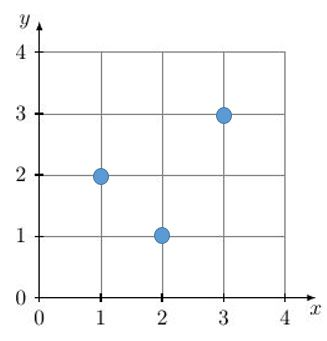
\includegraphics[width=7cm]{exam/final/least_square}
\end{figure}
\item
Let $\bm A$ be a matrix with \textit{linearly independent columns} and consider the \textit{projection matrix} $\bm P=\bm A(\bm A\trans\bm A)^{-1}\bm A\trans$. What are the possible eigenvalues for $\bm P$? Give your reasons.
\end{enumerate}
\newpage
\item \textbf{(20 points)} \\
True or False. No justifications are required.
\begin{enumerate}
\item
For real symmetric matrix $\bm A$, if $\bm A\succ 0$, then $\bm A^{-1}$ exists and $\bm A^{-1}\succ0.$\\
\item
If $\bm A$ is a matrix, (Note that $\bm A$ may not be real) then any element of the \textit{kernel} of $\bm A$ is \textit{perpendicular} to any element of the \textit{image} of $\bm A\trans$.\\
\item
The only $m\x n$ matrix of rank $0$ is $\bm 0$.\\
\item
Let $\bm A$ be real square matrix. If $\bm x$ is in $N(\bm A)$ and $\bm y$ is in $C(\bm A\trans)$, then $\bm x\bm y\trans=0.$\\
\item
If $\bm A$ and $\bm B$ are \textit{diagonalizable} matrices, then $\begin{bmatrix}
\bm A&\bm 0\\\bm 0&\bm B
\end{bmatrix}$ is \textit{diagonalizable}.
\end{enumerate}
\newpage
\item \textbf{(20 points)} \textit{SVD decomposition} \\
\begin{enumerate}
\item
Find the limiting values of $y_k$ and $z_k$ $(k\rightarrow\infty)$:
\[
\left\{
\begin{aligned}
y_{k+1}&=0.8y_k+0.3z_k,\\
z_{k+1}&=0.2y_k+0.7z_k,
\end{aligned}
\right.
\]
And $y_0=0,z_0=5.$\\
\textit{Hint: Show that $\begin{bmatrix}
0.8&0.3\\0.2&0.7
\end{bmatrix}$ is similar to $\begin{bmatrix}
0.5&0\\0&1
\end{bmatrix}.$}
\item
Find the SVD of the matrix $\begin{pmatrix}
0.5&0\\0&1
\end{pmatrix}.$
\end{enumerate}
\newpage
\item \textbf{(15+5 points)} \textit{Eigenvalues and Eigenvectors}\\
Given a \textit{real symmetric} matrix $\bm A$, the \emph{Rayleigh quotient} $R(\bm x)$ is defined as
\[
R(\bm x)=\frac{\bm x\trans\bm A\bm x}{\bm x\trans\bm x}\text{ for }\bm x\ne\bm0.
\]
Suppose the \textit{eigenvalues} of $\bm A$ are
$\lambda_1\le\lambda_2\le\dots\le\lambda_n$.
\begin{enumerate}
\item
Prove that the minimum eigenvalue $\lambda_1$ is the minimal value of $R(\bm x)$. 
\[
\text{i.e. }\lambda_1=\min_{\bm x\in\mathbb{R}^n-\{\bm 0\}}R(\bm x).
\]
\item
Suppose $\bm x_1$ is the eigenvector associated with $\lambda_1$, i.e. $\bm A\bm x_1=\lambda_1\bm x_1$.
\[
\text{Prove that }\lambda_2=\min_{\bm y\trans\bm x_1=0}R(\bm y).
\]
\item \textbf{(bonus question)}\\
Suppose $\bm v\in\mathbb{R}^n$ is an arbitrary given vector.
\[
\text{Prove that }\lambda_2\ge\min_{\bm y\trans\bm v=0}R(\bm y).
\]
\end{enumerate}
\newpage
\item \textbf{(10 points)} \textit{Positive semi-definite}\\
\begin{definition}[diagonal dominant]\qquad\\
A matrix $\bm M\in\mathbb{R}^{n\x n}$ is called \emph{diagonal dominant} if for $\forall i\in\{1,2,\dots,n\}$,
\[
|\bm M_{ii}|\ge\sum_{j\ne i}|\bm M_{ij}|.
\]
It is called \emph{strictly diagonal dominant} if for $\forall i\in\{1,2,\dots,n\}$,
\[
|\bm M_{ii}|>\sum_{j\ne i}|\bm M_{ij}|.
\]
\end{definition}
Prove the following statements:
\begin{enumerate}
\item
$\bm Z=\begin{pmatrix}
5&1&4\\1&5&3\\4&3&7
\end{pmatrix}$ is \textit{positive semi-definite}.
\item
If $\bm M$ is \textit{symmetric} and \textit{diagonal dominant}, then $\bm M\succeq0.$
\end{enumerate}
\end{enumerate}





